\section{美国FOF市场总资产建模}

\subsection{对资产对数增长率建立MA(5)模型}
首先利用ADF检验美国FOF总资产序列是否存在单位根, 在备择假设为平稳性的条件下, 对FOF基金的资产总量序列$\{ast\}$进行检验. 检验结果为$P=0.8158$, 这说明FOF的资产总量数据并不是一个平稳的时间序列. 而对FOF资产总量取对数差分后,即得到总资产的对数增长率序列$\{GR\_ast\}$,如图\ref{fig:unnamed-chunk-1-2}所示


\begin{figure}[h!]
	\centering
	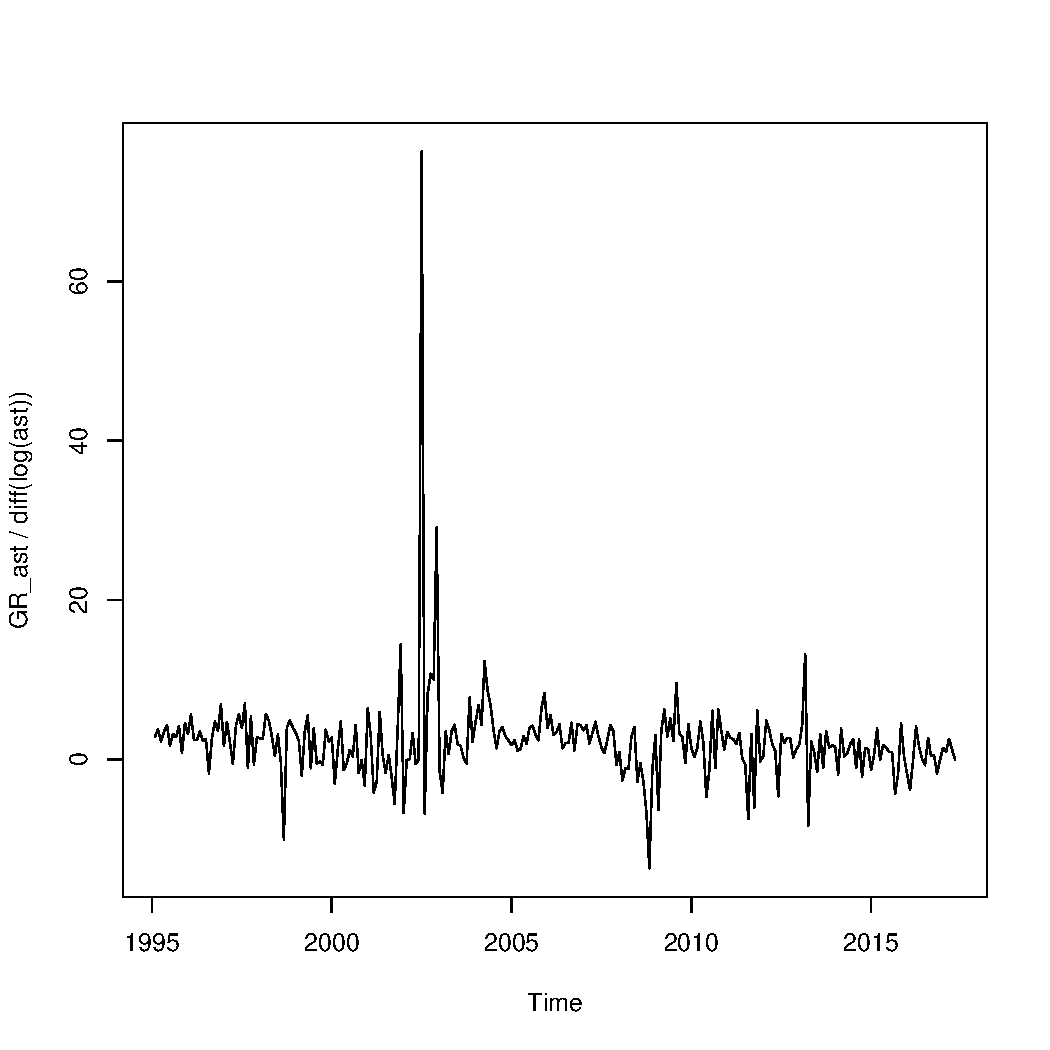
\includegraphics[width=0.6\linewidth]{pic/ast/unnamed-chunk-1-2}
	\caption{美国FOF基金总资产的对数增长率序列}
	\label{fig:unnamed-chunk-1-2}
\end{figure}
 再次进行ADF检验, 检验结果$P<0.01$, 拒绝了非平稳的原假设, 即其对数差分后是一个平稳序列.具体的R语言结果如下所示:
\begin{framed}
		 \begin{verbatim}
		 Augmented Dickey-Fuller Test
		 data:  ast
		 Dickey-Fuller = -1.4307, Lag order = 6, p-value = 0.8158
		 alternative hypothesis: stationary
		\end{verbatim}
	\end{framed}
\begin{framed}
	\begin{verbatim}
 	Augmented Dickey-Fuller Test 
   data:  GR_ast
   Dickey-Fuller = -4.9254, Lag order = 6, p-value = 0.01
   alternative hypothesis: stationary
	\end{verbatim}
\end{framed}
对对数差分后的序列进行ARMA建模. 见图\ref{gr_ast_ape}, 此序列的ACF函数在5阶处截尾, PACF函数在5阶处结尾,EACF显示应为MA(5) .
\begin{figure}[h!]
	\begin{minipage}[ht]{0.3\textwidth}
		\centering
		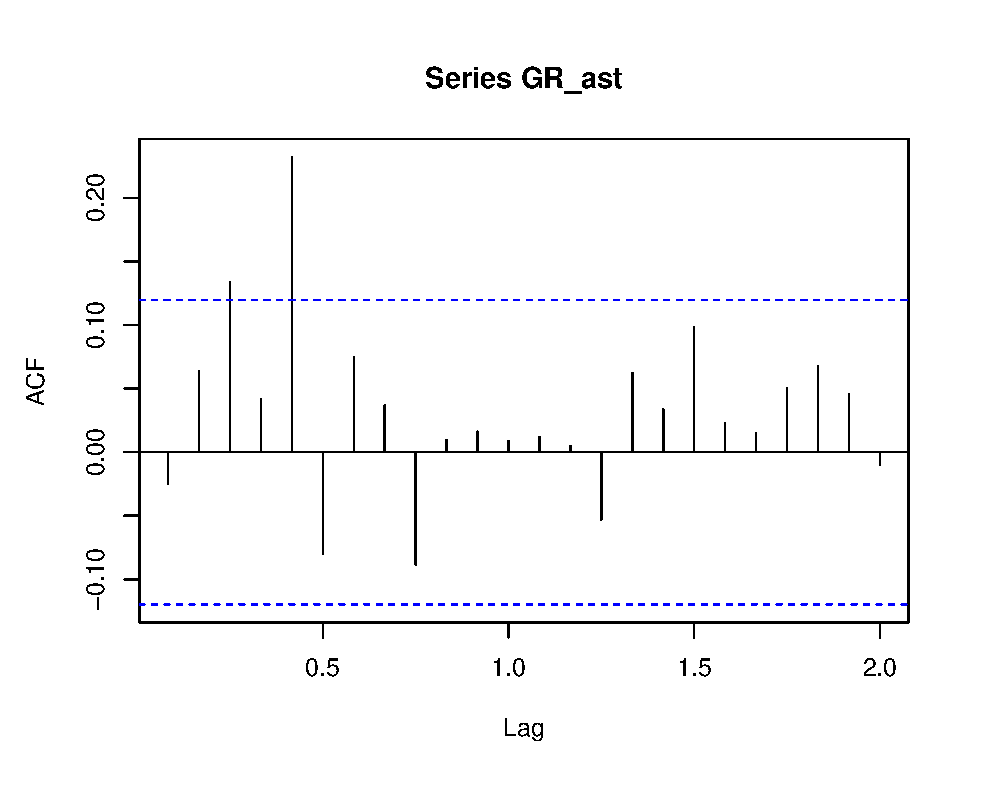
\includegraphics[width=\textwidth]{pic/ast/acf(gr_ast)}
		\subcaption{}\label{acf(gr_ast)}
	\end{minipage}%
	\hspace{0.04\textwidth}
	\begin{minipage}[ht]{0.3\textwidth}
		\centering
		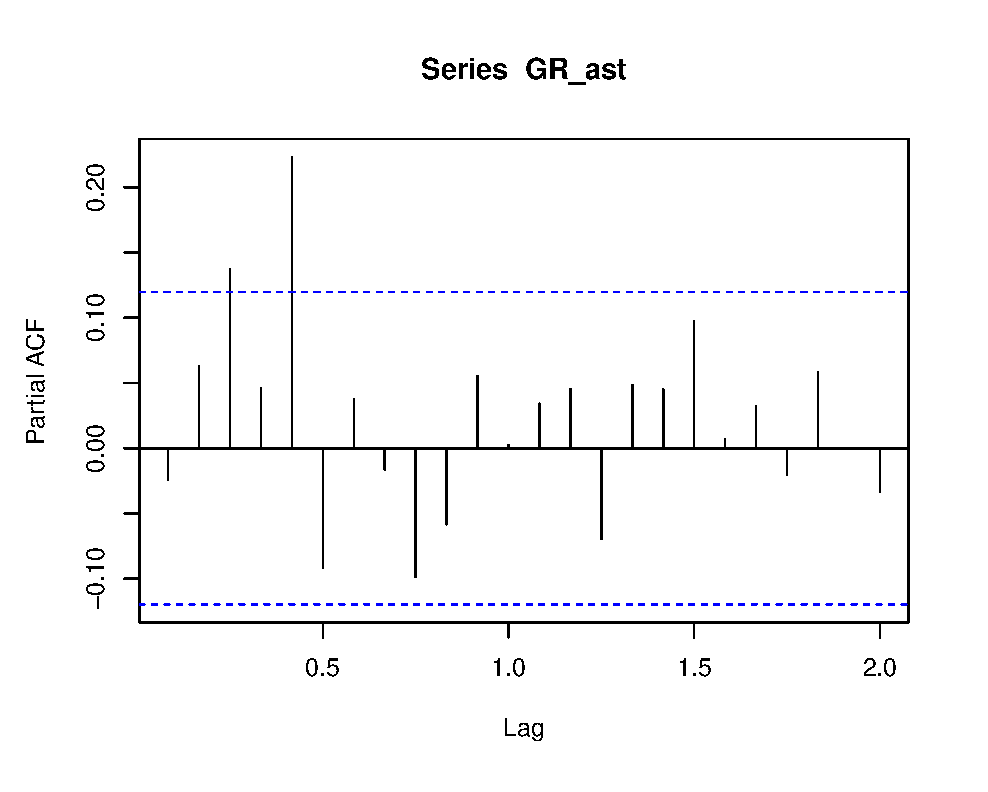
\includegraphics[width=\textwidth]{pic/ast/pacf(gr_ast)}
		\subcaption{}\label{pacf(gr_ast)}
	\end{minipage}
	\hspace{0.04\textwidth}
	\begin{minipage}[ht]{0.3\textwidth}
	\centering
	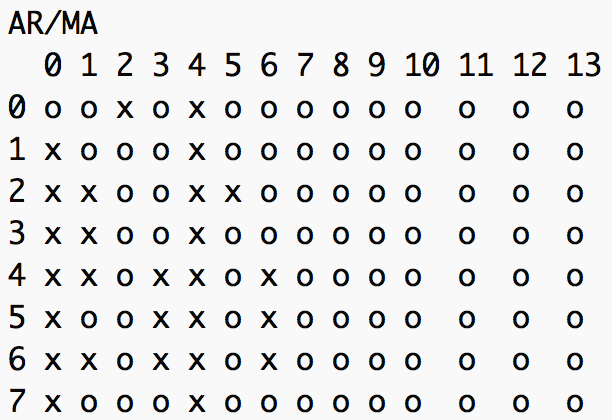
\includegraphics[width=1\textwidth]{pic/ast/eacf(gr_ast)}
	\subcaption{}\label{eacf(gr_ast)}
\end{minipage}
	\caption{GR\_ast序列的相关性: (a):ACF of GR\_ast; (b):PACF of GR\_ast; (c):EACF of GR\_ast}\label{gr_ast_ape}
\end{figure}
\emph{经过反复尝试,} 当使用MA(5)对序列进行刻画时, 可以得到较好的估计效果,且ma1,ma2和ma4都不显著,置0. MA(5)模型的极大似然估计结果如下:
\begin{framed}
\begin{verbatim}
 Call:
 arima(x = GR_ast, order = c(0, 0, 5), fixed = c(0, 0, NA, 0, NA, NA))
 Coefficients:
       ma1  ma2     ma3  ma4     ma5  intercept
         0    0  0.1352    0  0.2156     2.2333
 s.e.    0    0  0.0616    0  0.0556     0.4705
 sigma^2 estimated as 32.79:  log likelihood = -848.09,  aic = 1702.18
\end{verbatim}
\end{framed}





\subsection{模型诊断与异常值处理}

对上述模型的残差序列$r$进行Ljung-Box检验,如下:
\begin{framed}
\begin{verbatim} 
 	 	Box-Ljung test	 
 	 data:  r
 	 X-squared = 15.522, df = 22, p-value = 0.8389
\end{verbatim}
\end{framed}
$p-value=0.8389$ ,满足白噪声要求,说明$r$序列不存在一阶自相关.继续对残差$r$序列进行 McLeod.Li检验,见图\ref{mcr} ,检验结果各阶的$P$值都接近1, 说明不存在ARCH效应.具体的结果如图\ref{testr}所示,可以看到残差序列及残差平方序列的自相关性都很小,可以认为无自相关性.
\begin{figure}[h!]
	\begin{minipage}[ht]{0.31\textwidth}
		\centering
		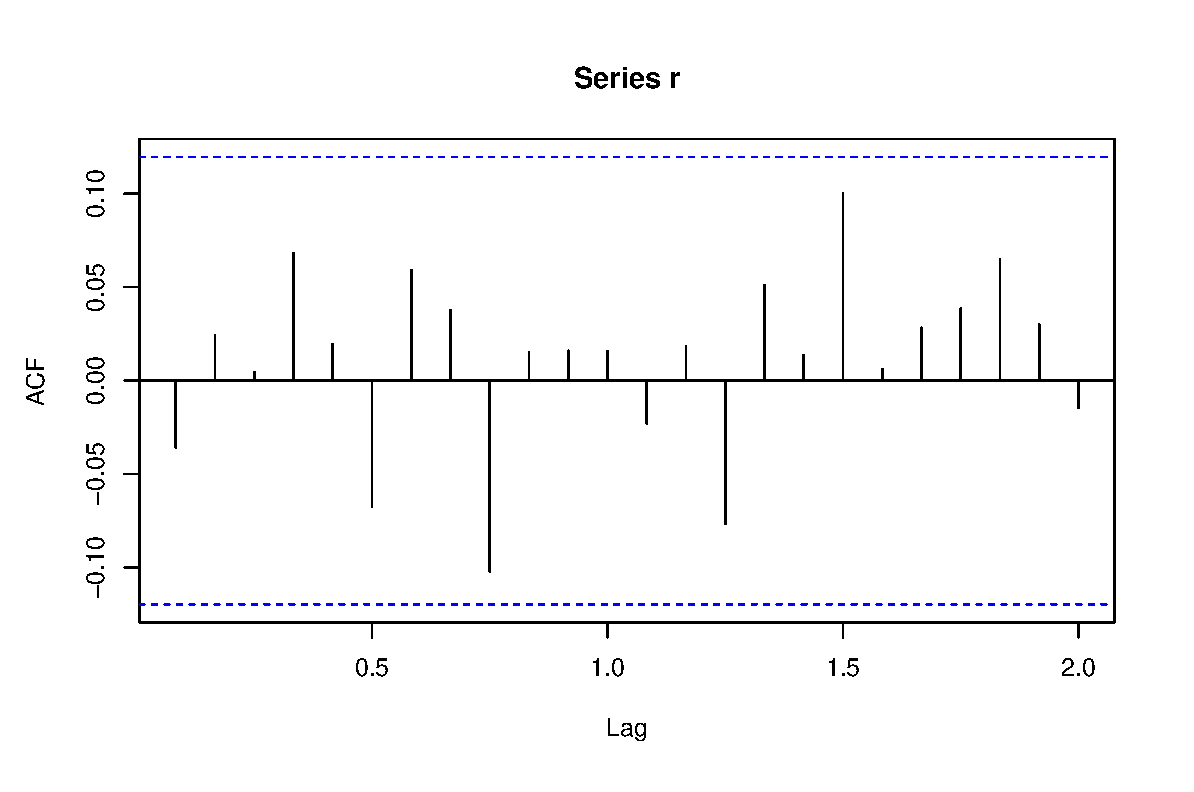
\includegraphics[width=\textwidth]{pic/ast/acfr}
		\subcaption{}\label{acfr}
	\end{minipage}%
	\hspace{0.02\textwidth}
	\begin{minipage}[ht]{0.31\textwidth}
		\centering
		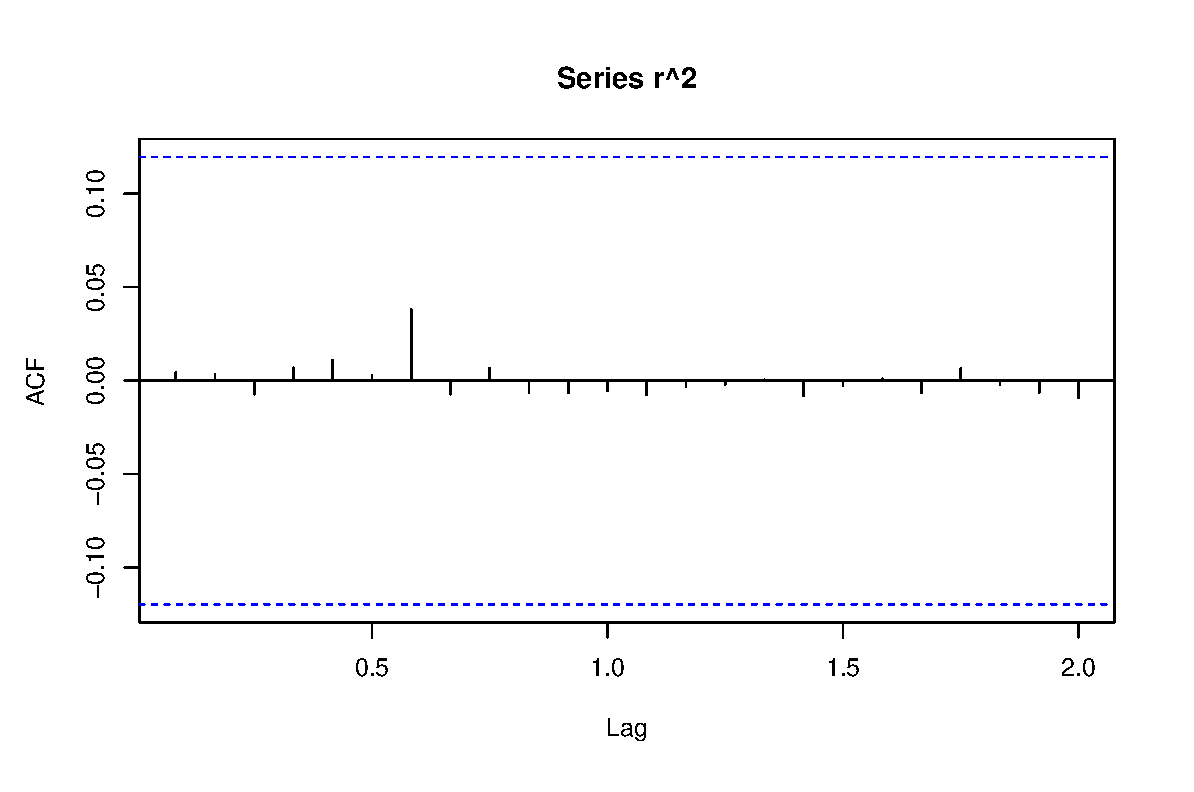
\includegraphics[width=\textwidth]{pic/ast/acfr2}
		\subcaption{}\label{acfr2}
	\end{minipage}
	\hspace{0.02\textwidth}
	\begin{minipage}[ht]{0.31\textwidth}
		\centering
		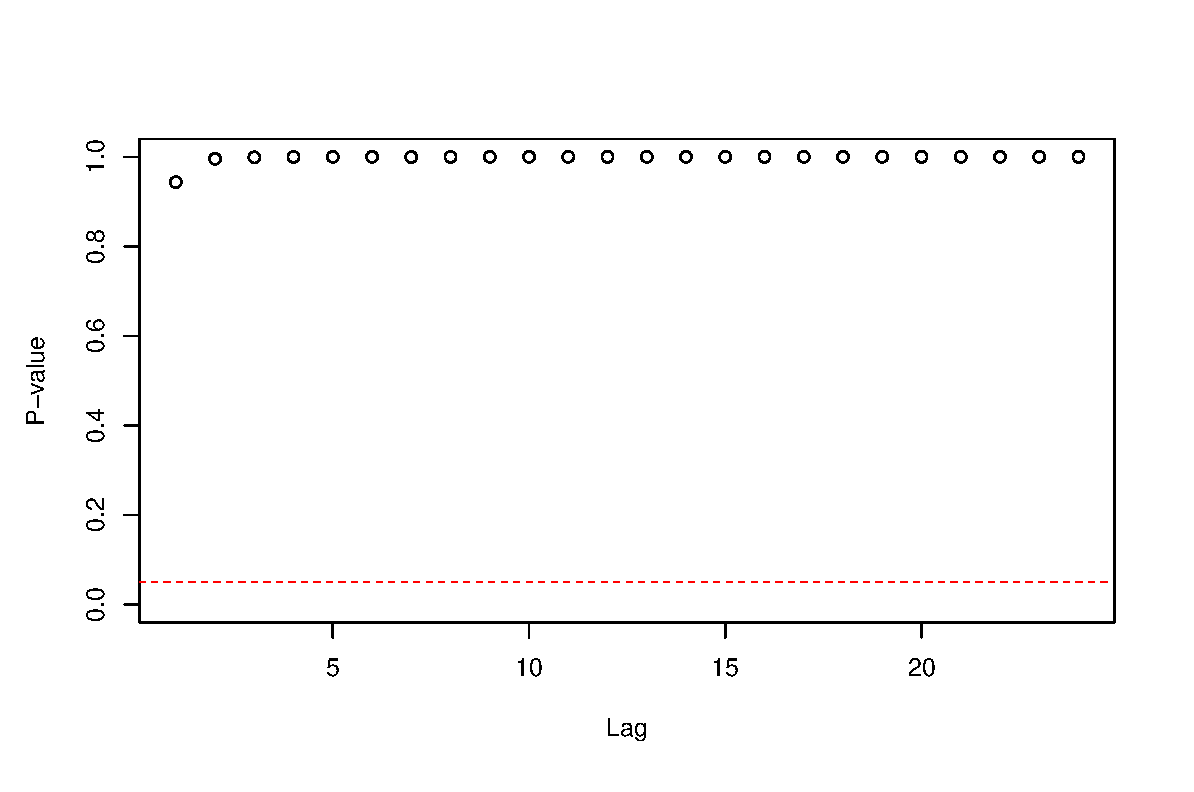
\includegraphics[width=1\textwidth]{pic/ast/mcr}
		\subcaption{}\label{mcr}
	\end{minipage}
	\caption{GR\_ast序列的MA(5)模型的残差序列相关性: (a):ACF of r; (b):ACF of r$^2$; (c):McLeod.Li.test of r}\label{testr}
\end{figure}

但进一步绘制出标准化的残差图, 见图\ref{fig:srgrast}
\begin{figure}
	\centering
	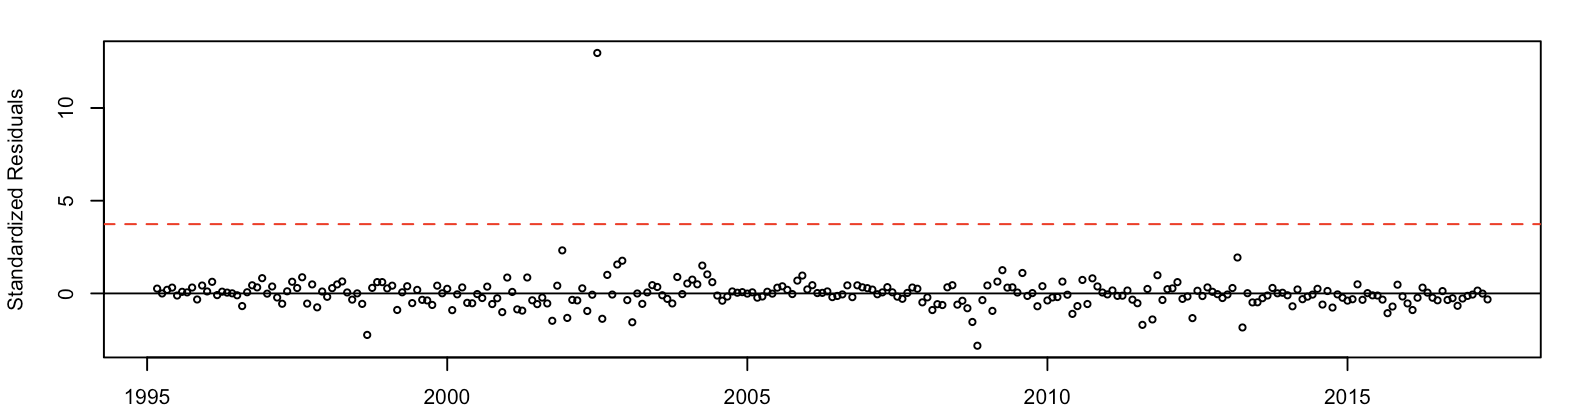
\includegraphics[width=0.8\linewidth]{pic/ast/srgr_ast}
	\caption{GR\_ast序列的MA(5) 模型的标准化残差}
	\label{fig:srgrast}
\end{figure}
发现在第90期有一个明显的异常值. 因为这个异常值的出现, 使得其他残差的尺度都会被缩小,很可能使得在模型诊断时,其他残差出现的波动聚类现象被忽略. 我们利用R语言中的detectIO()与detectAO()\footnote{其中IO和AO分别为新息异常值和可加异常值,具体原理的利用了 Chang, Chen and Tia在1998年提出的$\lambda_{1,T}$和$\lambda_{2,T}$统计量.}函数进行模型检测,也得到第90期为异常值的结果,且为IO异常值.为了削弱第90期的异常值对模型的影响, 令
\begin{equation}
GR\_ast[90] = \frac{1}{3} \cdot (GR\_ast[89]+GR\_ast[90]+GR\_ast[91])
\end{equation}
如图\ref{ioad}分别为原序列与进行异常值处理后的序列,从图\ref{ad}可看出波动有聚类现象.
\begin{figure}[h!]
	\begin{minipage}[ht]{0.48\textwidth}
		\centering
		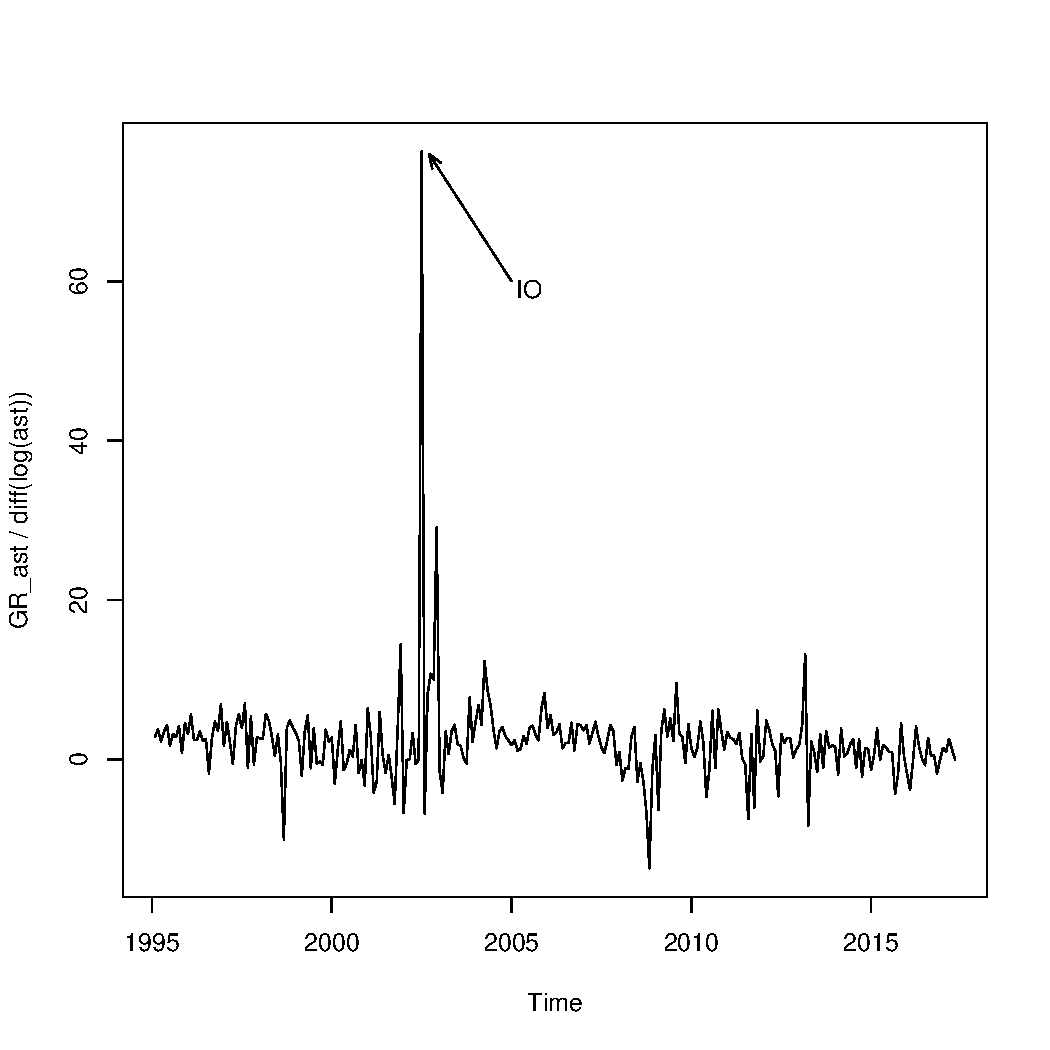
\includegraphics[width=0.7\textwidth]{pic/ast/unnamed-chunk-1-6}
		\subcaption{}\label{io}
	\end{minipage}%
	\hspace{0.04\textwidth}
	\begin{minipage}[ht]{0.48\textwidth}
		\centering
		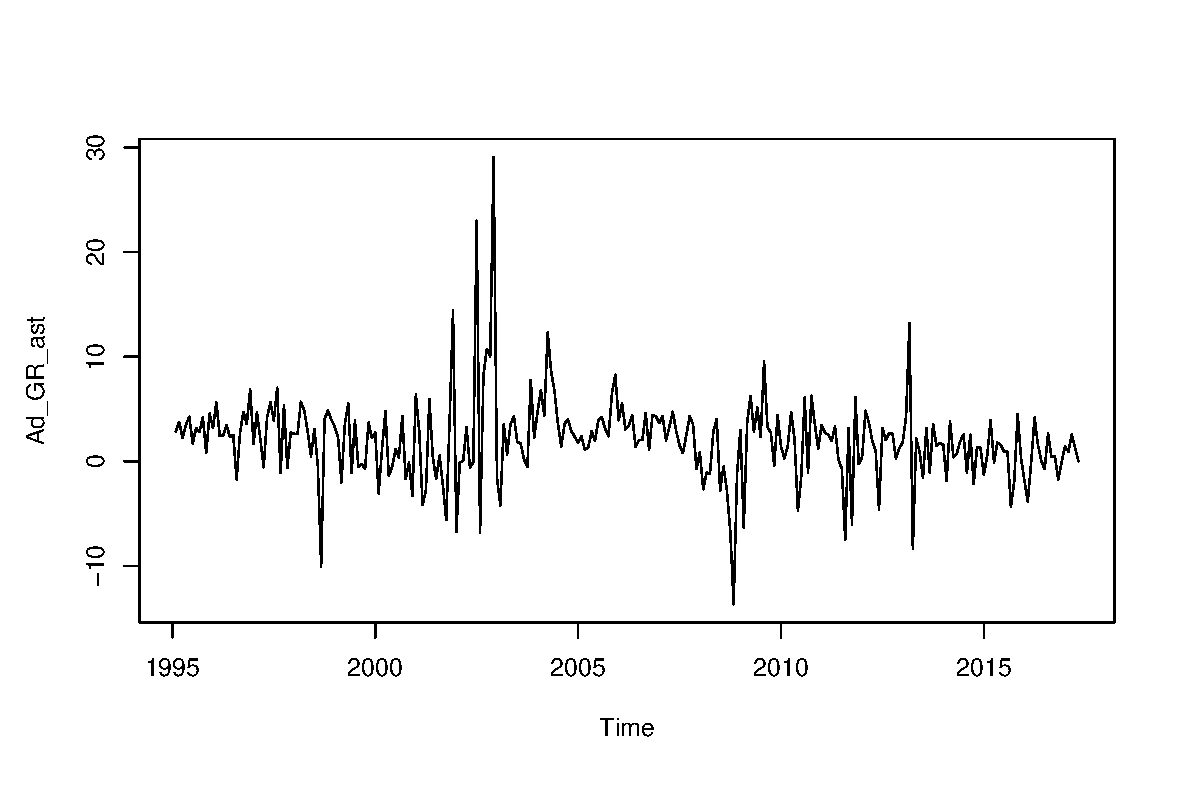
\includegraphics[width=\textwidth]{pic/ast/adgrast}
		\subcaption{}\label{ad}
	\end{minipage}
	\caption{进行异常值处理前后的GR\_ast序列: (a):未处理的GR\_ast序列; (b):进行异常值处理后的GR\_ast序列}\label{ioad}
\end{figure}






\subsection{对调整后的序列建立ARMA(0,5)-GARCH(1,1)模型}
序列进行异常值调整后,首先对其建立ARMA模型,与前面建立MA模型的方法一样,利用序列的ACF、PACF与EACF定阶,然后依旧建立了一个MA(5)模型,其参数的具体估计结果如下
\begin{framed}
\begin{verbatim} 
 Call:
 arima(x = Ad_GR_ast, order = c(0, 0, 5), fixed = c(0, 0, NA, 0, NA, NA))
 Coefficients:
       ma1  ma2     ma3  ma4     ma5  intercept
         0    0  0.1605    0  0.1671     2.0354
 s.e.    0    0  0.0591    0  0.0546     0.3171
 sigma^2 estimated as 15.4:  log likelihood = -746.78,  aic = 1499.56
\end{verbatim}
\end{framed}
对此模型的残差序列r2做Ljung-Box检验,结果如下:
\begin{framed}
\begin{verbatim}
 	Box-Ljung test
 data:  r2
 X-squared = 22.429, df = 22, p-value = 0.4345
\end{verbatim}
\end{framed}
对其残差做McLeod.Li检验,见图\ref{fig:mcr2},可见所有前24阶的p值都在0.05内,其原假设为残差平方序列无相关性,则拒绝原假设.
\begin{figure}[h!]
	\centering
	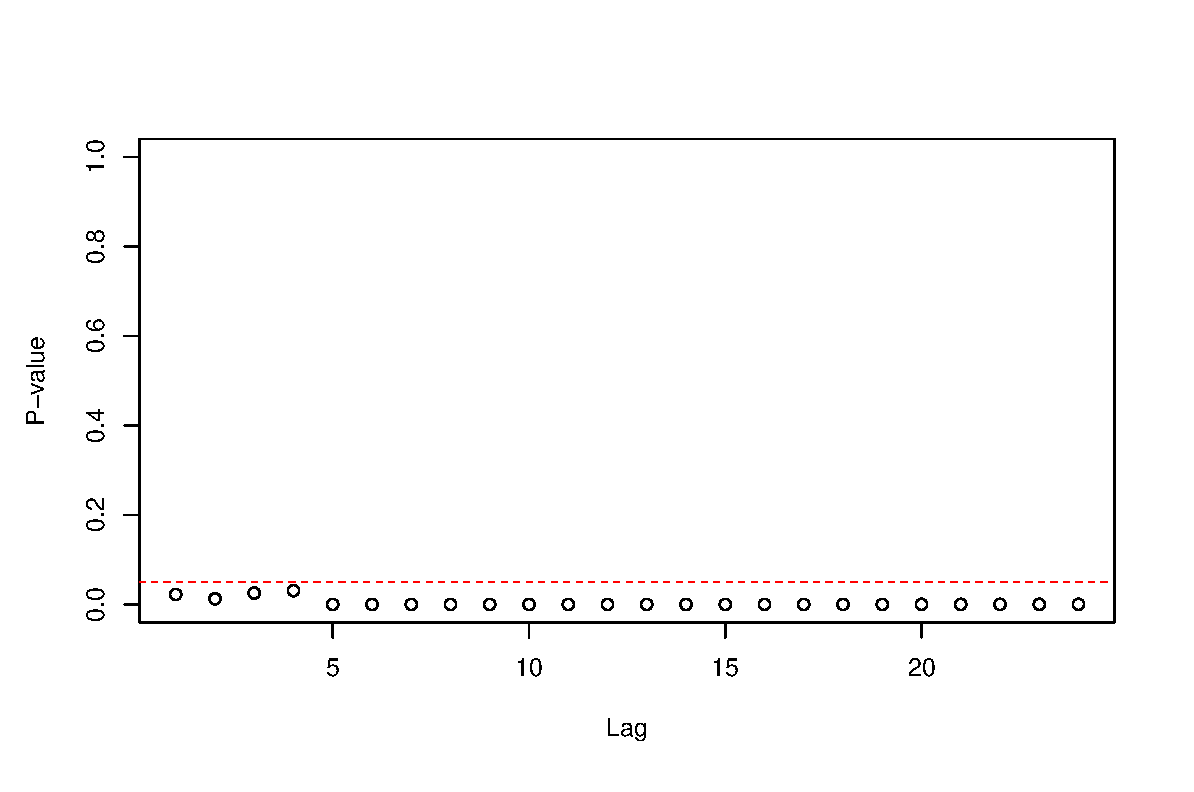
\includegraphics[width=0.5\linewidth]{pic/ast/mcr2}
	\caption{调整后序列的MA模型残差的McLeod.Li检验}
	\label{fig:mcr2}
\end{figure}
即现在的残差存在ARCH效应,需进一步建立异方差模型.利用rugarch包里的函数,建立MA(5)-GARCH(1,1)模型,残差分布为学生t分布.具体的参数估计结果如下(其中ma4不显著,置0):

\begin{framed}
	\begin{verbatim}
	 *---------------------------------*                         
	 *          GARCH Model Fit        *                           
	 *---------------------------------*
	 GARCH Model	: sGARCH(1,1)
	 Mean Model	: ARFIMA(0,0,5)
	 Distribution	: std 
	 ------------------------------------
	         Estimate  Std. Error  t value Pr(>|t|)
	 mu      2.198557    0.221154   9.9413 0.000000                                  
	 ma1     0.077369    0.067282   1.1499 0.250177
	 ma2     0.074749    0.058956   1.2679 0.204838
	 ma3     0.079972    0.050914   1.5707 0.116245
	 ma4     0.000000          NA       NA       NA
	 ma5     0.119163    0.050347   2.3668 0.017941
	 omega   5.250380    3.087206   1.7007 0.089001
	 alpha1  0.619542    0.378827   1.6354 0.101960
	 beta1   0.379458    0.151319   2.5077 0.012153
	 shape   2.897172    0.762001   3.8021 0.000143
	\end{verbatim}
\end{framed}
对模型进行诊断,见图\ref{fig:diagarch},
\begin{figure}[h!]
	\centering
	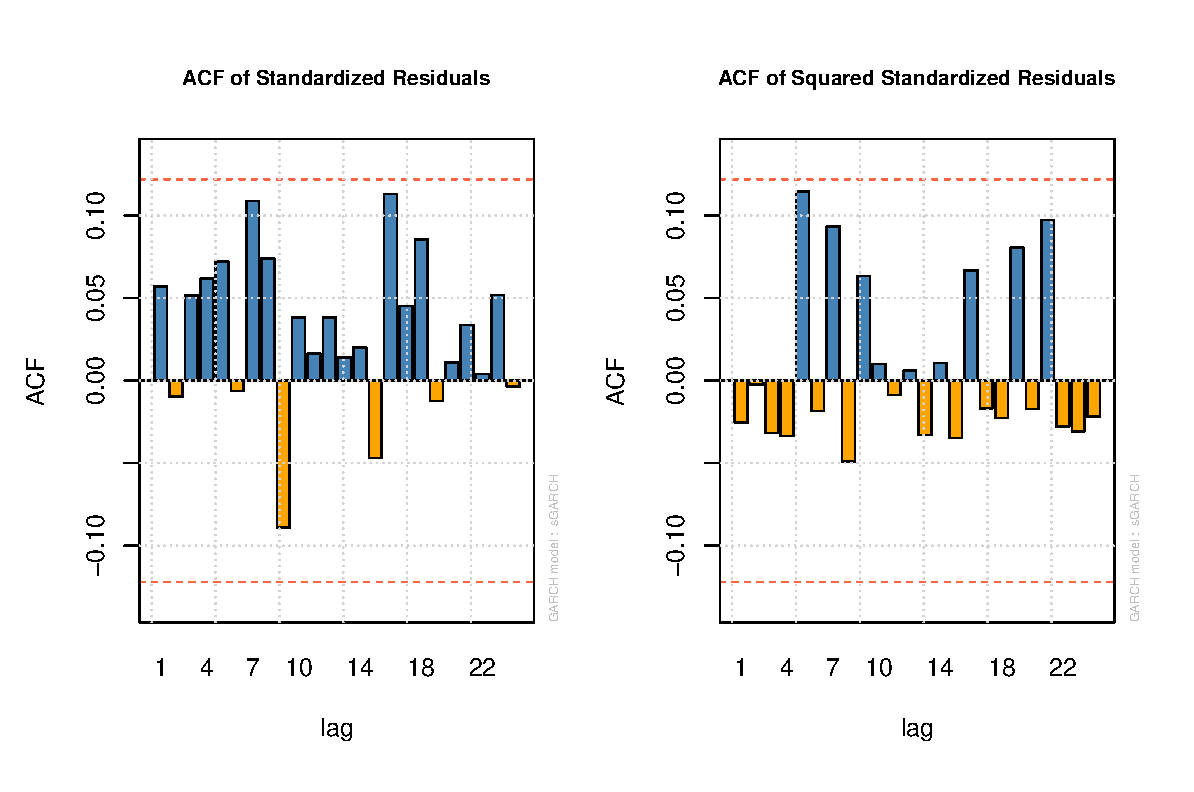
\includegraphics[width=0.7\linewidth]{pic/ast/diagarch}
	\caption{ARMA-GARCH模型诊断:左为标准化残差的ACF,右为标准化残差平方的ACF}
	\label{fig:diagarch}
\end{figure}
\begin{figure}[h!]
	\centering
	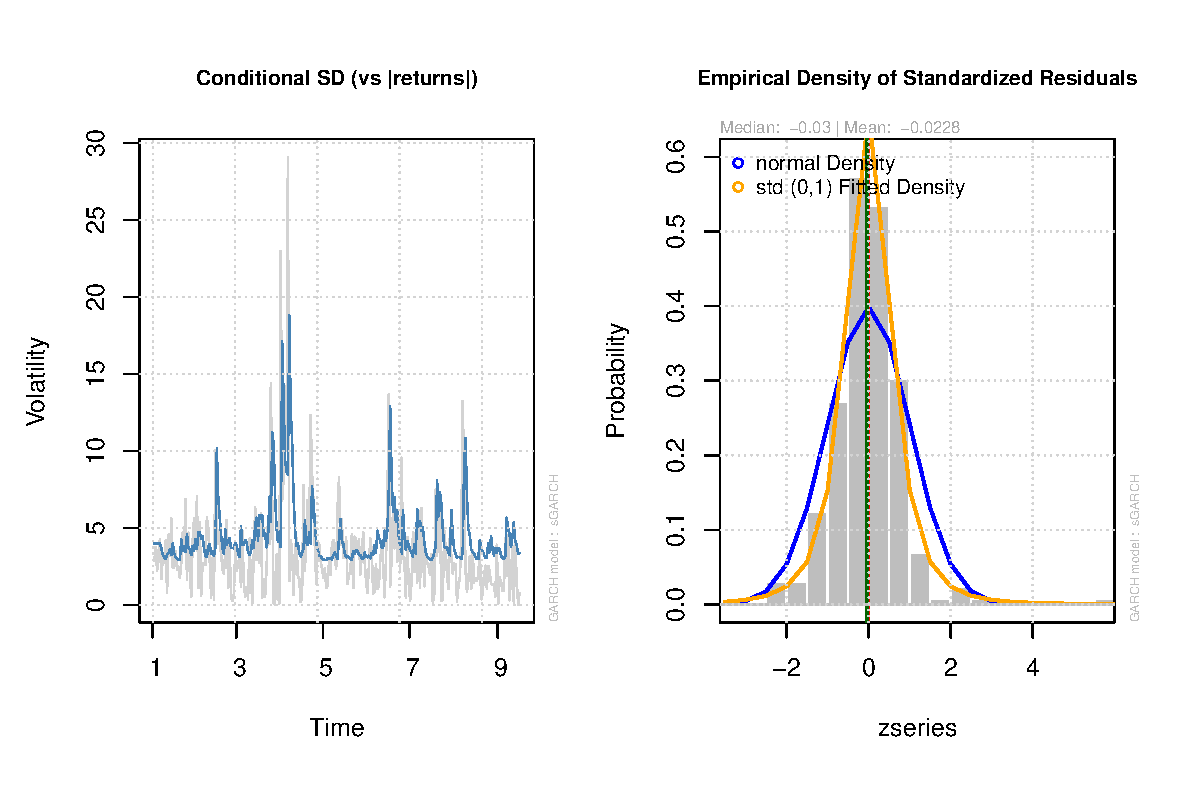
\includegraphics[width=0.6\linewidth]{pic/ast/diav}
	\caption{ARMA-GARCH模型诊断:左为模拟的残差波动与真实残差比较,右为模拟残差的std分布与标准正态分布比较}
	\label{fig:diav}
\end{figure}
可以直观看到其标准化残差不再具有一阶与二阶自相关性,这一点也可由GARCH模型结果中的Ljung-Box Test on Standardized Residuals,Ljung-Box Test on Standardized Squared Residuals和ARCH LM Tests的统计结果看到,具体可以运行附录里code即可重现,这里不再赘述.这说明现在的ARMA(0,5)-GARCH(1,1)模型是充分的.进一步见图\ref{fig:diav},可以看到对残差的t分布假设是合适的,其尾部比标准正态分布要厚,说明了FOF基金资产的对数增长率的波动,即风险,也存在尖峰厚尾的现象.
\begin{figure}[h!]
	\begin{minipage}[ht]{0.48\textwidth}
		\centering
		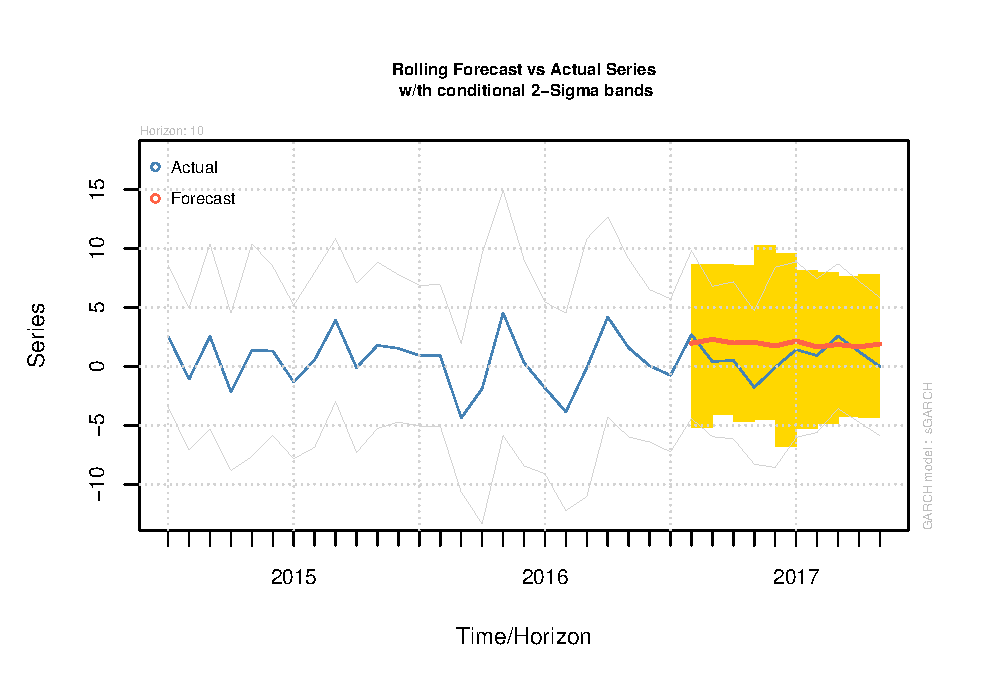
\includegraphics[width=\textwidth]{pic/ast/fastroll}
		\subcaption{}\label{fastroll}
	\end{minipage}%
	\hspace{0.04\textwidth}
	\begin{minipage}[ht]{0.48\textwidth}
		\centering
		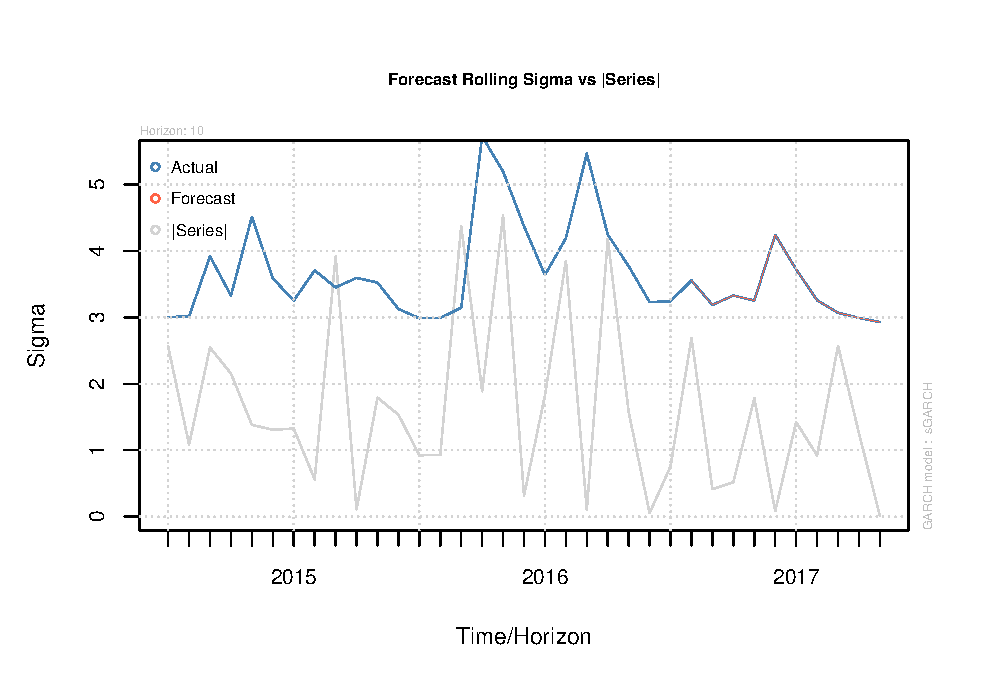
\includegraphics[width=\textwidth]{pic/ast/fastrollv}
		\subcaption{}\label{fastrollv}
	\end{minipage}
	\caption{利用ARMA(0,5)-GARCH(1,1)模型对调整后的FOF资产对数增长率及其波动方差进行滚动预测: (a):FOF资产对数增长率预测; (b):波动方差的滚动预测} \label{f}
\end{figure}
\par 现在可以利用上述模型进行预测分析如图\ref{f}所示,是序列值与序列波动方差的滚动预测,可以看到,对数增长率的预测相比与真实序列,较为平缓,但能有效反映出真实值的趋势,对预测未来值波动方向具有指导意义.对方差的预测,与真实值也符合的较好,能够反映出波动的大致方向.